\section{Introduction}
The extended tractability of the AMPLE program for globular and transmembrane protein targets through the use of residue-residue contact predictions to restrain \textit{ab initio} structure prediction was highlighted in \cref{chap:proof_of_principle}. However, the study explored exclusively the metapredictor PCONSC2 for globular targets without considering any alternatives. It thus served solely as proof of principle for applications of contact predictions in unconventional \gls{mr}.

Besides the individual contact prediction algorithms employed by the PCONSC2 protocol, numerous metapredictors have been developed exploiting different combinations of starting alignments and individual contact predictors to identify the strongest correlating pairs for optimal contact prediction \cite{Kamisetty2013-le,Skwark2014-qp,Jones2015-vq,Ma2015-vo,He2017-fn,Michel2017-pm,Wang2017-rx}. Furthermore, each of those protocols typically includes its own post-prediction algorithms to find a consensus amongst individual predictions and/or further identify patterns characteristic for residue pairings between secondary structure elements in a protein fold. Thus, depending on the overall protocol, the resulting predictions may differ significantly despite the same underlying algorithms to generate starting alignments and to predict residue contact pairs.

Furthermore, the precision of contact predictions used as distance restraints in \textit{ab initio} structure prediction improves the accuracy of the folding process significantly. However, a diversity of structure prediction protocols, whether fragment-based or not, have been applied and each with a unique integration of contact information as distance restraints \cite{Marks2011-os,Michel2014-eg,Adhikari2015-lb,Jones2015-vq,Ovchinnikov2015-tn,Adhikari2018-lj}. Such divergence results in three major problems: (1) researchers cannot directly compare results, and thus have to test each protocol against their own with every newly published approach; (2) novice users might find it difficult to make appropriate decisions given the diversity of algorithms and lack of comparative studies; and (3) users only interested in the information encoded in predicted contact pairs are at risk of picking the most readily available approach over the most accurate for their problem.

Thus, the presented work was aimed at extensively comparing state-of-the-art contact prediction and \textit{ab initio} protein structure prediction protocols with a focus on the use of such resulting decoys in unconventional \gls{mr}, with a particular focus on AMPLE users.

\section{Materials \& Methods}
\subsection{Target selection of PREDICTORS dataset} \label{sec:methods_dataset_predictors}
This study was conducted using 18 out of 27 targets in the PREDICTORS dataset (\cref{sec:methods_dataset_predictors}). All nine targets with PFAM alignment depths of less than 100 were excluded (\cref{table:appendix_dataset_predictors}).

\subsection{Contact prediction}
Residue contacts for each target sequence were predicted using three different metapredictors, namely METAPSICOV \cite{Jones2015-vq}, GREMLIN \cite{Kamisetty2013-le}, and PCONSC2 \cite{Skwark2014-qp}. Web servers for METAPSICOV v2016-02 (\url{http://bioinf.cs.ucl.ac.uk/METAPSICOV}) and GREMLIN v2015-12 (\url{http://gremlin.bakerlab.org}) were used to retrieve two sets of contact predictions. Web servers were preferred in this study over local installations to best imitate the typical behaviour of AMPLE users. Both servers were used with default settings.

The GREMLIN web server returns the raw contact prediction files as well as pre-formatted ROSETTA distance restraints. The raw contact prediction files were downloaded to allow different contact selection thresholds as well as local conversion into ROSETTA restraints files. The METAPSICOV web server returned two contact prediction files, one after STAGE1 and another after STAGE2 post-prediction processing. In this study, contact predictions after STAGE1 (referred to as METAPSICOV from here onwards) were chosen. The PCONSC2 contact prediction set was obtained using a local installation of PCONSC2 due to downtime of the web server at the time of this study. The settings and databases were identical to \cref{sec:ample_proof_conpred}. Additionally to the three main contact predictions outlined above, a set of BBCONTACTS restraints was obtained for protein targets containing \textbeta-strands (\cref{sec:methods_bbcontacts_addition}).

The sequence-database versions of all three metapredictors, whether on- or offline, were identical to those outlined in \cref{sec:ample_proof_methods}.

\subsection{Contact-to-restraint conversion} \label{subsec:ample_predicotrs_con2res}
Contact restraints for \textit{ab initio} protein structure prediction were generated by selecting the top-ranking contact pairs from each prediction and reformatting them into a ROSETTA-readable format. The number of top-ranking contact pairs varied according to the two energy functions used (FADE cutoff: \textit{L}; SIGMOID cutoff: 3\textit{L}/2; where \textit{L} corresponds to the number of residues in the protein chain). Both energy functions are sigmoidal functions and introduced into the ROSETTA folding protocol in the same fashion. 

Neither energy function enforces a specified distance between restrained atoms but reward those that meet it. The two energy functions (\cref{fig:ample_predictors_efuncs}) differ in that the FADE function does not only have an upper but also a lower bound. Based on previous findings \cite{Michel2014-eg, Skwark2014-qp}, the FADE function was set to acknowledge a formed restraint if the participating C\textbeta\ atoms (C\textalpha\ in case of Gly) were within 9\AA. In comparison, the SIGMOID function was defined with amino acid specific distances for C\textbeta\ atoms (C\textalpha\ in case of Gly) to recognise the different sizes of each amino acid \cite{Kamisetty2013-le, Ovchinnikov2015-tn}.

\begin{figure}[H]
    \centering
    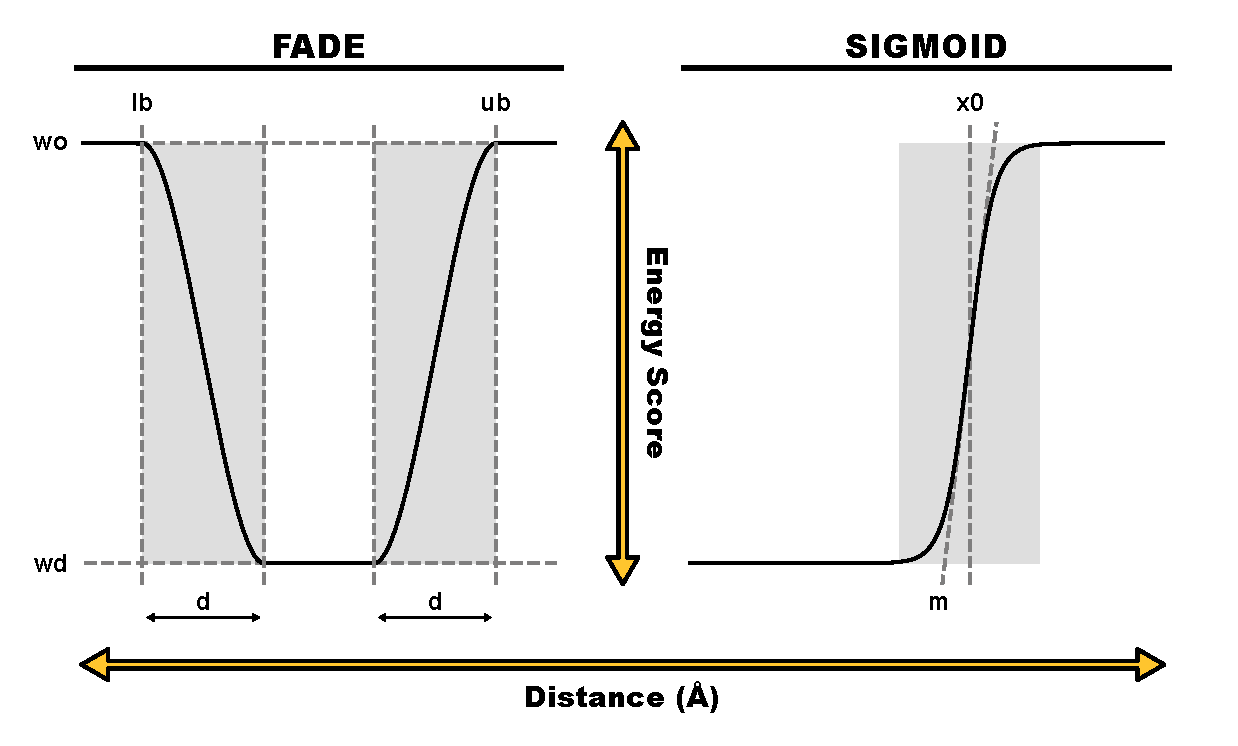
\includegraphics[width=\textwidth]{ample_predictors_efuncs.pdf}
    \caption[Schematic comparison of ROSETTA energy functions]{Schematic comparison of two ROSETTA energy functions. Abbreviations corresponds to input parameters.}
    \label{fig:ample_predictors_efuncs}
\end{figure}

To explore the effects of the varying ROSETTA energy function definitions, six separate contact restraint lists were created for each \textalpha-helical target and nine for each \textbeta-structure containing target. The top-ranking contact pairs per prediction were converted using the PCONSFOLD definition of the FADE function \cite{Michel2014-eg}, the GREMLIN definition of the SIGMOID function \cite{Ovchinnikov2015-tn}, and additionally the PCONSC2+BBCONTACTS definition of the FADE function for \textbeta-structure containing targets (\cref{sec:bbcontacts_addition}).

The conversion was handled in AMPLE and invoked with the keywords outlined in \cref{table:ample_predictors_kwargs}. The \texttt{-restraints\_factor} keyword defines the factor used to select contact pairs based on the target chain length, i.e. a factor of 1.5 would correspond to 3\textit{L}/2 contact pairs. The \texttt{-distance\_to\_neighbour} keyword defines the minimum distance in sequence space between contact pair participating residues, which were set to 5 residues for the FADE function \cite{Michel2014-eg} and 3 for the SIGMOID function \cite{Ovchinnikov2015-tn}. Additionally, all distance restraints were given an additional weight when introduced via the SIGMOID energy function to balance its energy term with all remaining terms in the ROSETTA scoring function (Sergey Ovchinnikov, personal communication). This was achieved by using the \texttt{-restraints\_weight} keyword and weights of 1.0 and 3.0 for the FADE and SIGMOID energy functions.

The addition of BBCONTACTS to existing sets of contacts was achieved with the FADE function in an identical manner as described in \cref{sec:bbcontacts_addition}. In comparison, the \texttt{SCALARWEIGHTED} term in the GREMLIN implementation of the SIGMOID energy function \cite{Ovchinnikov2015-tn} was multiplied by the number of occurrences of each contact pair in the combined map.

\begin{table}[H]
    \centering
    \caption[AMPLE keyword arguments for two ROSETTA energy functions]{AMPLE keyword arguments for FADE and SIGMOID ROSETTA energy functions.}
    \label{table:ample_predictors_kwargs}
    \begin{tabularx}{\textwidth}{ s b }
        \hline
        \textbf{Energy Function} & \textbf{AMPLE keywords} \\
        \hline
        \multirow{6}{1em}{FADE} & \texttt{-contact\_file <FILENAME>} \\
                                & \texttt{-contact\_format <FORMAT>} \\
                                & \texttt{-energy\_function FADE} \\
                                & \texttt{-restraints\_factor 1.0} \\
                                & \texttt{-distance\_to\_neighbour 5} \\
                                & \texttt{-restraints\_weight 1.0} \\
        \hline
        \multirow{6}{1em}{FADE (BBCONTACTS)} & \texttt{-contact\_file <FILENAME>} \\
                                & \texttt{-contact\_format <FORMAT>} \\
                                & \texttt{-energy\_function FADE} \\
                                & \texttt{-restraints\_factor 1.0} \\
                                & \texttt{-distance\_to\_neighbour 5} \\
                                & \texttt{-restraints\_weight 1.0} \\
        \hline
        \multirow{6}{1em}{SIGMOID} & \texttt{-contact\_file <FILENAME>} \\
                                & \texttt{-contact\_format <FORMAT>} \\
                                & \texttt{-energy\_function SIGMOID} \\
                                & \texttt{-restraints\_factor 1.5} \\
                                & \texttt{-distance\_to\_neighbour 3} \\
                                & \texttt{-restraints\_weight 3.0} \\
        \hline
        \multirow{6}{1em}{SIGMOID (BBCONTACTS)} & \texttt{-contact\_file <FILENAME>} \\
                                & \texttt{-contact\_format <FORMAT>} \\
                                & \texttt{-energy\_function SIGMOID\_bbcontacts} \\
                                & \texttt{-restraints\_factor 1.5} \\
                                & \texttt{-distance\_to\_neighbour 3} \\
                                & \texttt{-restraints\_weight 3.0} \\
        \hline
    \end{tabularx}
\end{table}

\subsection{\textit{Ab initio} protein structure prediction}
Six or nine individual lists of contact restraints generated for each target were used in separate ROSETTA \textit{ab initio} protein structure prediction runs. Additionally, protein structures were predicted without any predicted contact restraints to acquire a control decoy set. Homologous fragments were excluded during fragment library generation to imitate the folding process of a target with unknown fold. Fragment libraries were generated for each target using a local installation of ROSETTA v2015.22.57859. PSIPRED secondary structure predictions were included from contact prediction runs and provided via the \texttt{-psipredfile} option. In total, 1,000 \textit{ab initio} decoys were generated per run using ROSETTA v2015.22.57859 with default settings \cite{Rohl2004-dj} and one of the seven or ten (six/nine plus control) contact conditions described in \cref{subsec:ample_predicotrs_con2res}. In total, 162 sets of models were generated across 18 protein targets.

\subsection{Molecular Replacement}
Besides considering decoy quality, one key interest of this study was the assessment of the decoy sets created in the previous step as \textit{ab initio} \gls{mr} search model templates. To reduce the enormous computational cost linked to trialling 162 decoy sets, 108 sets were chosen from the following conditions: simple ROSETTA, PCONSC2 prediction and FADE function, GREMLIN prediction and SIGMOID function, METAPSICOV prediction and FADE function, and where applicable, PCONSC2+BBCONTACTS, GREMLIN+BBCONTACTS and METAPSICOV+BBCONTACTS predictions and FADE function. Overall, this resulted in four \gls{mr} runs for the six \textalpha-helical targets, seven runs for the six all-\textbeta, and seven runs for the six mixed \textalpha-\textbeta\ targets. The resulting 108 model sets were trialled in AMPLE v1.1.0 and CCP4 v7.0.28. Structure solution success was assessed as described in \cref{sec:methods_mr_success}.

\section{Results}
\subsection{Direct comparison of three contact metapredictors}
In this study, a direct comparison between three metapredictors --- GREMLIN, METAPSICOV and PCONSC2 --- was carried out. Residue-residue contact pairs were predicted for 18 protein target sequences with a range of chain lengths and numbers of effective sequences in their PFAM \gls{msa}s.

METAPSICOV was the most precise contact predictor across the protein target dataset in this study (\cref{fig:ample_predictors_cutoff}). The difference between the three metapredictors was most evident in the highest-scoring contact pairs (\textit{L}/10). The median precision values for METAPSICOV and PCONSC2 contact predictions were above 50\% up to \textit{L} contact pairs. GREMLIN, in comparison, predicted contacts with a median precision score at least 20\% worse than that of METAPSICOV and 15\% worse than PCONSC2. However, at 3\textit{L}/2 contact pairs the median precision scores were much more similar across the three different metapredictors: METAPSICOV and PCONSC2 were near identical, and GREMLIN is at most 12\% worse compared to the other two. Inspecting the mean precision scores over a continuous range of selection cutoff values illustrated further the difference between METAPSICOV, PCONSC2 and GREMLIN (Fig \ref{fig:ample_predictors_covprc}). The former two similarly high precision scores compared to the average precision scores for GREMLIN, which were approximately 0.2 precision score units lower. Added to the difference in precision scores was the difference in sequence coverage (\cref{fig:ample_predictors_covprc}). Although producing the on-average worst contact predictions out of the three metapredictors, GREMLIN contact predictions had the highest sequence coverage. However, an analysis of singleton contact pairs, usually with high degrees of \gls{fp} predicted contacts, revealed a positive correlation ($\rho_{Pearson}=0.47$; $p<0.001$) between the fraction of singleton contact pairs and sequence coverage and hinted to a weak negative correlation ($\rho_{Pearson}=-0.27$; $p<0.05$) between the fraction of singleton contact pairs and contact precision (\cref{fig:ample_predictors_singletons}).

\begin{figure}[H]
    \centering
    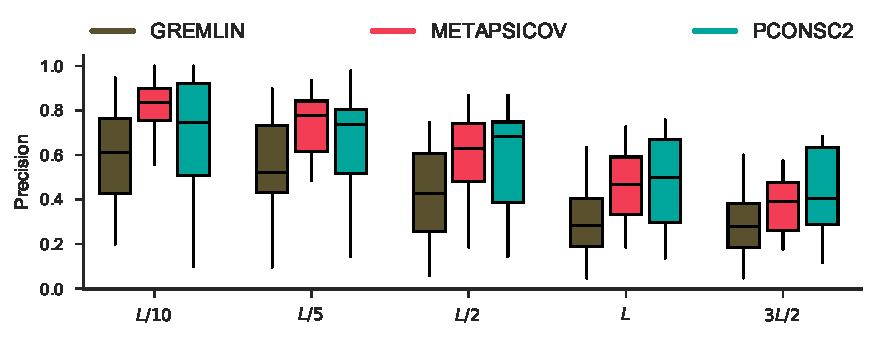
\includegraphics[width=\textwidth]{ample_predictors_cutoff.pdf}
    \caption[Precision analysis of three metapredictors]{Distribution of precision values for three metapredictors computed at five contact selection cutoff values relative to the target chain length (\textit{L}).}
    \label{fig:ample_predictors_cutoff}
\end{figure}

\begin{figure}[H]
    \centering
    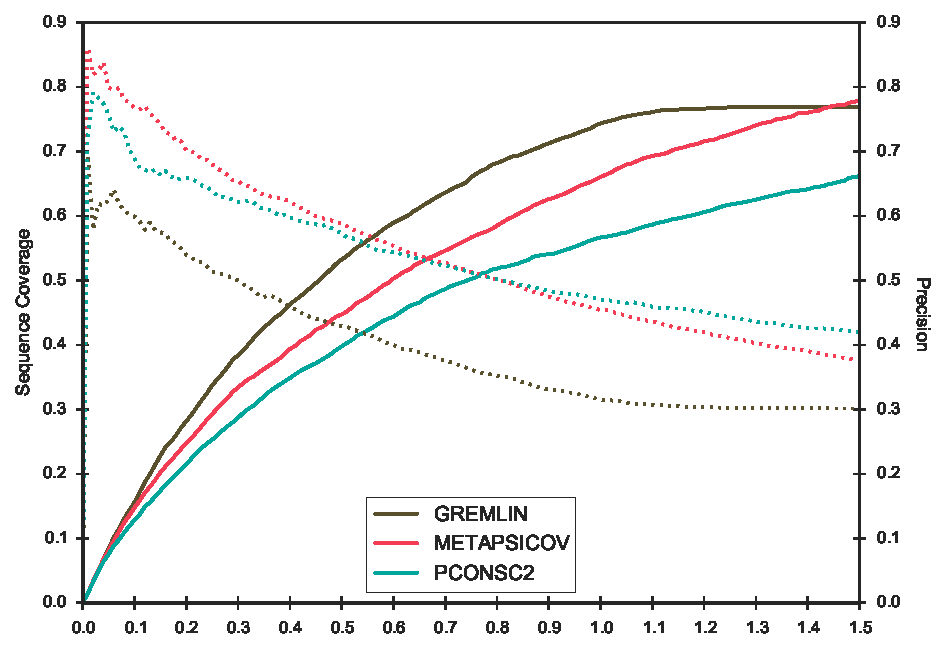
\includegraphics[width=\textwidth]{ample_predictors_covprc.pdf}
    \caption[Sequence coverage and contact precision analysis]{Average sequence coverage (line) and contact prediction precision scores (dashed) across a continuous range of contact selection cutoffs ranging from $[0.0, 1.5]$ for all targets.}
    \label{fig:ample_predictors_covprc}
\end{figure}

\begin{figure}[H]
    \centering
    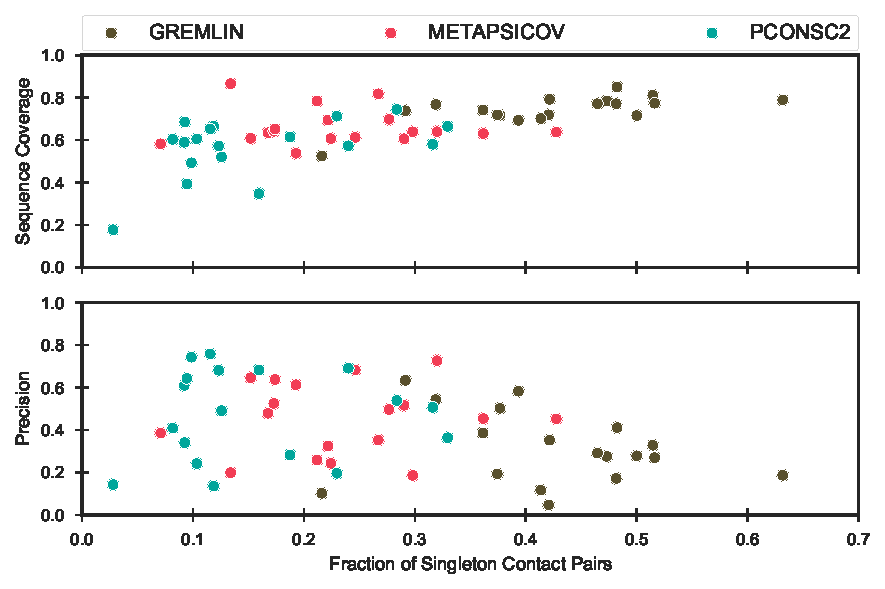
\includegraphics[width=\textwidth]{ample_predictors_singletons.pdf}
    \caption[Contact singleton analysis for three metapredictors]{Contact singleton analysis compared against the precision of top-\textit{L} contact pair lists for three metapredictors.}
    \label{fig:ample_predictors_singletons}
\end{figure}

Given that the overall precision of contact pairs predicted by the three metapredictors differed, it was important to understand where the difference originated. To investigate this, a comparison of the precision values at different cutoff levels on a per-target basis was performed. For the majority of targets the precision scores were very similar across the three metapredictors (\cref{fig:ample_predictors_prcpeaks}). However, the prediction precision of some targets differed significantly. For example, the METAPSICOV prediction for the human retinoic acid nuclear receptor HRAR (\gls{pdb}: 1fcy) contained high precision in its highest scoring (top-\textit{L}/10) contact pairs (\cref{fig:ample_predictors_prcpeaks}). In comparison, GREMLIN and PCONSC2 predictions for the same target contained less precise contact pairs (\textDelta \textsubscript{METAPSICOV-GREMLIN} $L/10=-0.522$; \textDelta \textsubscript{METAPSICOV-PCONSC2} $L/10=-0.435$). However, the addition of further contact pairs up to 3\textit{L}/2 resulted in near-identical precision across the three metapredictors for this target. A second example illustrating such a difference were the contact predictions for the human galectin-3 CRD sequence (\gls{pdb}: 4lbj). In contrast to the previous example, the data showed high precision scores for the METAPSICOV and PCONSC2 predictions for this target, yet low precision for the top GREMLIN contact pairs (\textDelta \textsubscript{METAPSICOV-GREMLIN} $L/10=-0.231$; \textDelta \textsubscript{METAPSICOV-PCONSC2} $L/10=0.077$). 

\begin{figure}[H]
    \centering
    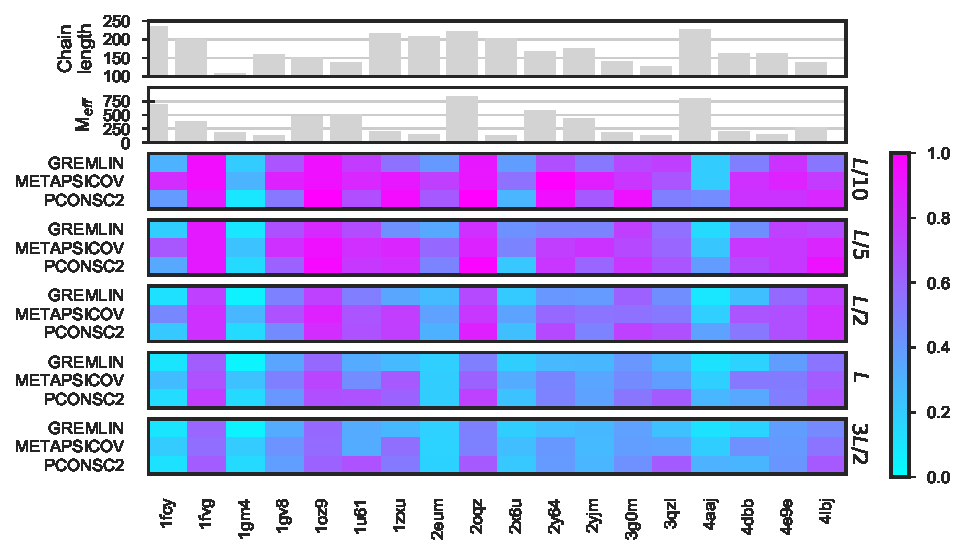
\includegraphics[width=\textwidth]{ample_predictors_prcpeaks.pdf}
    \caption[Comparison of contact precision for three metapredictors]{Contact prediction precision scores from three metapredictors for 18 targets at different contact pair selection thresholds (\textit{L}, which is the target chain length). The PFAM alignment depth is given by means of \gls{meff}. The colour scale corresponds to the precision in range $[0, 1]$.}
    \label{fig:ample_predictors_prcpeaks}
\end{figure}

The data presented in \cref{fig:ample_predictors_prcpeaks} also indicated that there was no direct link between chain length or \gls{meff} and the precision of the resulting contact predictions. The N-(5'-phosphoribosyl)anthranilate isomerase sequence (\gls{pdb}: 4aaj) with a chain length of 228 residues and 750 effective sequences in its PFAM \gls{msa} yielded a mean precision at \textit{L}/10 contact pairs of 0.283 (top-\textit{L}: 0.195) across the three metapredictors. This strongly contrasted with the sequence of sortase B (\gls{pdb}: 2oqz), which showed similar characteristics yet obtained  mean precision at \textit{L}/10 contact pairs of 0.938 (top-\textit{L}: 0.622).

Although the contact predictions differed in precision, an interesting question rested with the similarity of the predicted contact pairs amongst the sets. Thus, the similarity of contact predictions across the three metapredictors was an important metric to evaluate the most appropriate algorithm for AMPLE users. Using the Jaccard similarity index to evaluate the direct overlap of contact pairs across sets of predictions, the data suggested very little similarity between the contact predictions of the three metapredictors for each target (\cref{fig:ample_predictors_jaccardidx}). As with the differences in precision scores at higher cutoff thresholds, the Jaccard index was also lower --- indicating less overlap --- at higher cutoff thresholds. However, it is worth noting that the Jaccard index only considers identical matches and did not consider the neighbourhood of a contact pair. Thus, the index does not highlight similar regions with contact pairs in both maps.

\begin{figure}[H]
    \centering
    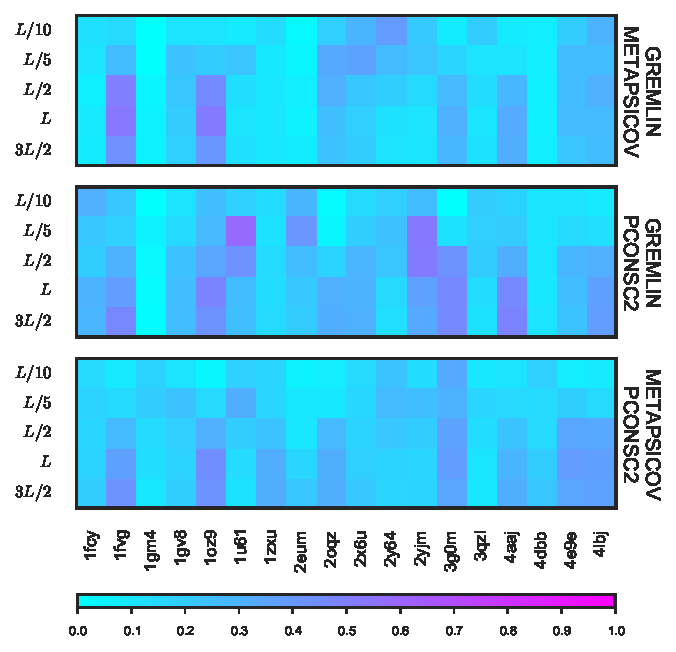
\includegraphics[width=0.8\textwidth]{ample_predictors_jaccardidx.pdf}
    \caption[Metapredictor contact pair similarity analysis]{Jaccard similarity index illustrates a higher degree of overlap between metapredictor contact predictions with increasing numbers of contact pairs included in the calculation. The three panels show the different comparisons. The color scale corresponds to the Jaccard index in range $[0, 1]$.}
    \label{fig:ample_predictors_jaccardidx}
\end{figure}

\subsection{Protein structure prediction with two ROSETTA energy functions}
The accuracy of the starting decoys is a major factor for an AMPLE run to succeed \cite{Thomas2017-sh}. Thus, the quality of the decoys was of great essence to this study. Given the two different ROSETTA energy functions, FADE and SIGMOID, all predicted contacts were subjected to individual \textit{ab initio} structure prediction runs. Additionally, all contact predictions were enriched with BBCONTACTS for all \textbeta-containing targets in separate trials. A total of 234,000 individual decoys were generated in this study across all targets, contact predictions and ROSETTA energy function combinations.

Separating these individual decoys solely by the ROSETTA energy function (excluding unrestrained ROSETTA decoys) showed that the FADE energy function resulted in marginally more accurate decoys (median TM-score FADE: 0.3541; median TM-score SIGMOID: 0.2969). To further investigate which energy function was more suitable for the target dataset, the decoy sets were grouped by two additional characteristics: the fold of the target, and the source of distance restraints used. The results strongly suggested that the FADE energy function results in more accurate decoy sets (\cref{fig:ample_predictor_tmmedian}), outperforming the SIGMOID energy function by median TM-score in two-thirds of all decoys sets (FADE: 58; SIGMOID: 32). A split of the decoy sets into separate categories by fold and the addition of BBCONTACTS revealed that the SIGMOID energy function only yields similar results for all-\textbeta\ targets in combination with BBCONTACTS-supported distance restraints. Although the total count of decoy sets with higher accuracies between the two energy functions in this category were similar, the actual differences in TM-scores further supported the strength of the FADE energy function compared to the SIGMOID.

Besides the structure prediction accuracy of each set of decoys, the single, most accurate decoy is also of great interest. If one energy function consistently predicted single decoys more accurately, it might be appropriate to reconsider the structure identification routine (i.e. clustering) in AMPLE for search model preparation. However, a similar difference to that of the decoy quality of entire sets was observed for the top-1 decoy in each set (\cref{fig:ample_predictor_tmtop}). The FADE energy function outperformed the SIGMOID function for the majority of target-contact prediction combinations (FADE: 51; SIGMOID: 39). However, the GREMLIN distance restraints in combination with the SIGMOID energy function produced better top-1 decoys than GREMLIN restraints with the FADE energy function. This suggested that GREMLIN restraints and the SIGMOID energy function were tailored to complement each other with the ultimate goal of predicting single decoys to high accuracy over entire sets of decoys. Additionally, the spread of decoy quality differences between the two energy functions widens when only looking at the best decoy in each predicted set (\textDelta Median \gls{tmscore}\textsubscript{ALL}: $min=0.002, max=0.429$; \textDelta Median \gls{tmscore}\textsubscript{TOP}: $min=0.002, max=0.456$). 

\begin{figure}[H]
    \centering
    \begin{subfigure}[b]{0.90\textwidth}
        \centering
        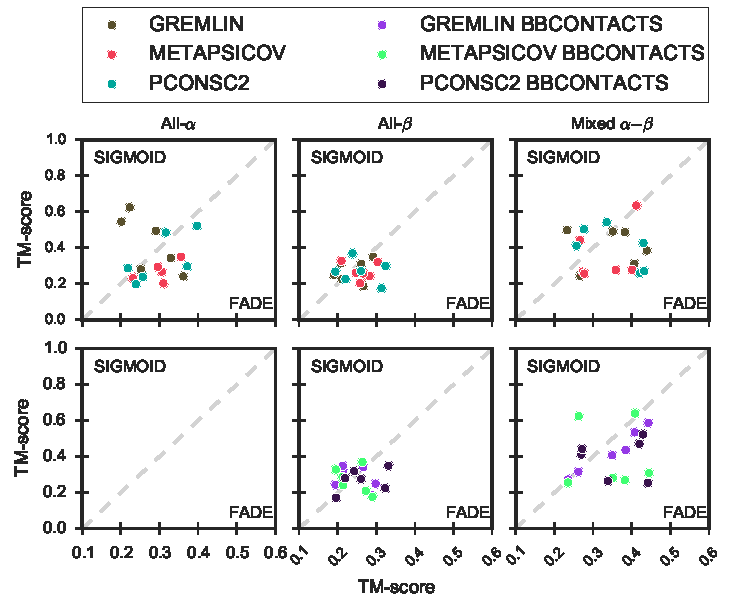
\includegraphics[width=\textwidth]{ample_predictors_tmmedian.pdf}
        \caption{}
        \label{fig:ample_predictor_tmmedian}
    \end{subfigure}

    \begin{subfigure}[b]{0.90\textwidth}
        \centering
        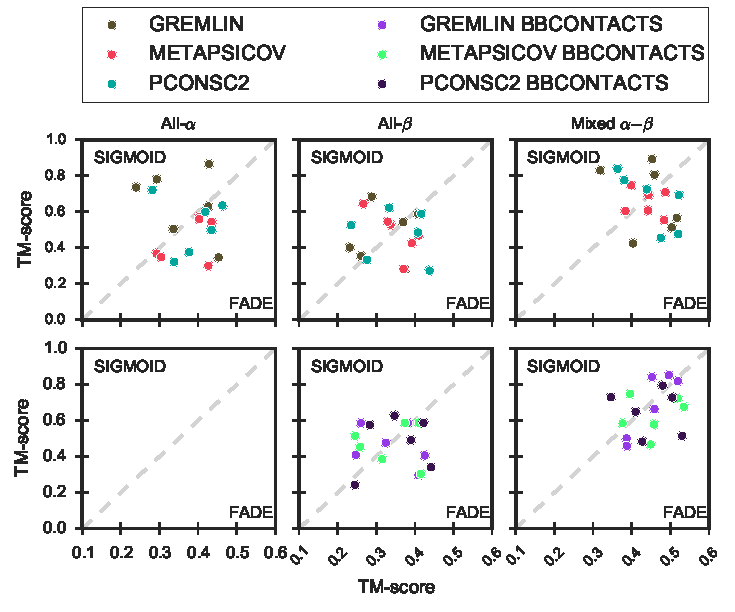
\includegraphics[width=\textwidth]{ample_predictors_tmtop.pdf}
        \caption{}
        \label{fig:ample_predictor_tmtop}
    \end{subfigure}
    \caption[TM-score comparison between ROSETTA energy functions]{(a) Median and (b) top-1 decoy TM-score comparison of FADE and SIGMOID ROSETTA energy functions differentiated by fold and the addition of BBCONTACTS restraints.}
\end{figure}

A \gls{kde} of TM-scores using each predicted decoy was generated with the TM-scores of individual decoys separated only by fold class and ROSETTA energy function (\cref{fig:ample_predictor_tmdensity}). This density estimate further supported the results presented above: the FADE energy function generated more accurate decoys. However, a very important detail was highlighted by the \gls{kde}s. Distinct regions with high density are visible in the estimates of the TM-scores of individual decoys for all-\textalpha\ and mixed \textalpha-\textbeta\ targets (\cref{fig:ample_predictor_tmdensity}). The bimodal distribution of decoy TM-scores from both energy functions strongly suggested that predicted structures were either native-like or not (based on the TM-score threshold of $\leq0.5$). However, the number of correctly predicted decoys versus incorrectly predicted decoys was in favour of the latter. The decoy sets of all-\textbeta\ targets did not show such distinct regions of high density for decoys with TM-scores of less than 0.5 in any of its \gls{kde}s (\cref{fig:ample_predictor_tmdensity}). The generally poor decoy quality of decoys predicted without any predicted distance restraint information (ROSETTA) highlighted the benefit of contact predictions to \textit{ab initio} protein structure prediction.

\begin{figure}[H]
    \centering
    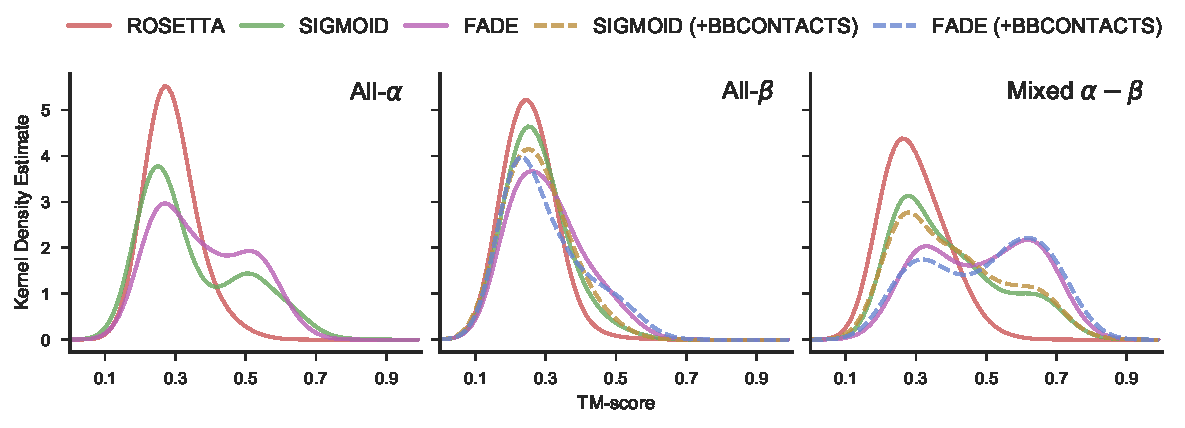
\includegraphics[width=\textwidth]{ample_predictors_tmdensity.pdf}
    \caption[TM-score distribution by fold category and ROSETTA energy function]{\Gls{kde}s of TM-scores of all decoys in each respective fold class separating by ROSETTA energy function (SIGMOID or FADE) and no contact information used (ROSETTA). Dashed lines indicate decoys which were predicted with the addition of BBCONTACTS predictions.}
    \label{fig:ample_predictor_tmdensity}
\end{figure}

A further important aspect of the presented work is the demonstration of the benefits of BBCONTACTS prediction addition to the \textit{ab initio} protein structure prediction of \textbeta-containing targets. Although previous results described in \cref{chap:proof_of_principle} in combination with those presented above outlined overall improvements in decoy quality, it was essential to understand which targets benefit from this treatment. Figure \ref{fig:ample_predictor_bbdir} highlights the effects of adding BBCONTACTS restraints to the structure prediction strategies employed here. In summary, the addition of BBCONTACTS restraints hardly affecte the decoy quality of most targets under the various contact prediction and energy function combinations. Nevertheless, three target, contact prediction and energy function combinations yielded TM-score improvements of at least 0.1 TM-score units compared to the same condition without the addition of BBCONTACTS restraints. In contrast, the addition of BBCONTACTS restraints did not lower the median TM-score by more than 0.1 for any target (\cref{fig:ample_predictor_bbdif}).

\begin{figure}[H]
    \centering
    \begin{subfigure}[b]{\textwidth}
        \centering
        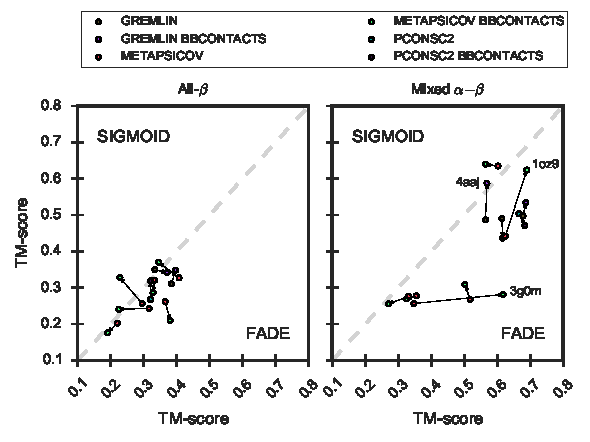
\includegraphics[width=0.9\textwidth]{ample_predictors_bbdir.pdf}
        \caption{}
        \label{fig:ample_predictor_bbdir}
    \end{subfigure}
    
    \begin{subfigure}[b]{\textwidth}
        \centering
        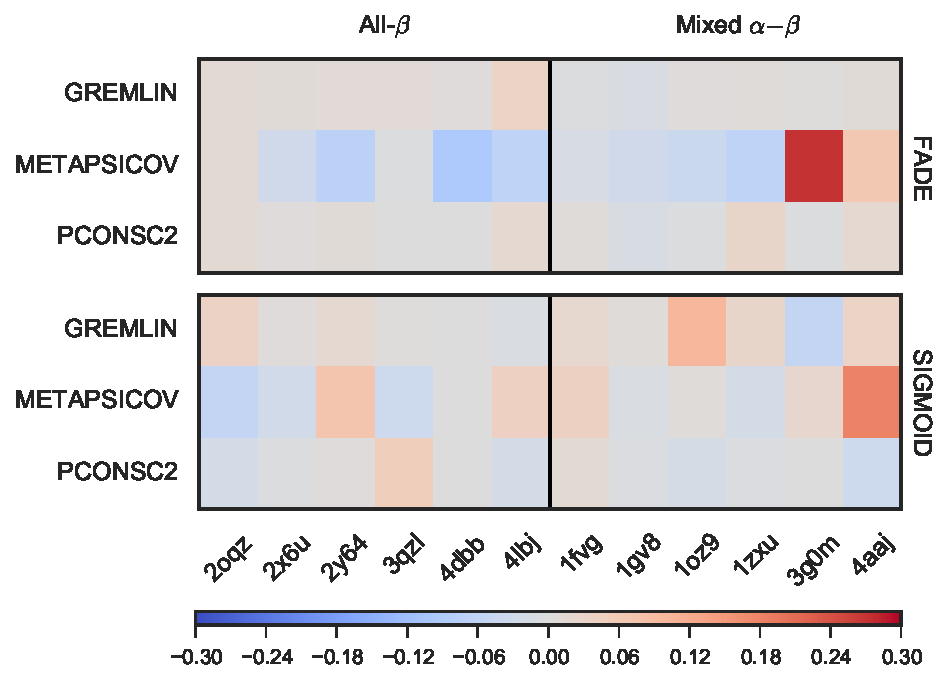
\includegraphics[width=0.8\textwidth]{ample_predictors_bbdif.pdf}
        \caption{}
        \label{fig:ample_predictor_bbdif}
    \end{subfigure}

    \caption[Median TM-score analysis by fold category and ROSETTA energy function]{Median TM-score comparison of FADE and SIGMOID ROSETTA energy functions differentiated by fold (excl. all-\textalpha). (a) Arrows indicate the effect on decoy quality through the addition of BBCONTACTS restraints. Targets with a distance $<0.03$ TM-score units between normal and BBCONTACTS-added conditions were excluded from the scatter plots. (b) Effect on decoy quality through the addition of BBCONTACTS restraints highlighted by heatmap difference. The color scale corresponds to the difference in median TM-score between normal and BBCONTACTS-added contact maps.}
\end{figure}

Two further aspects in understanding the differences in effects of the FADE and SIGMOID ROSETTA energy functions on decoy quality were the target chain length and restraints precision. The former appeared to affect the final decoy quality of all 1,000 decoys insignificantly (\cref{fig:ample_predictor_tmsummary}). However, the restraint precision resulted in some differences between the two ROSETTA energy functions (\cref{fig:ample_predictor_tmsummary}). The FADE energy function (top-\textit{L} restraints) generally appeared to be less sensitive to restraint lists with higher \gls{fp} contact pairs.  In contrast, the SIGMOID function  (3\textit{L}/2 restraints) produced less accurate decoys than the FADE function with more accurate restraints. Most strikingly, the FADE energy function generated decoys with a median TM-score of 0.678 for the N-(5'-phosphoribosyl)anthranilate isomerase domain (\gls{pdb}: 4aaj) compared to the SIGMOID function with a median TM-score of 0.498. Nevertheless, both energy functions appeared to broadly follow a positive linear trend, i.e. better restraint precision resulted in more accurate decoys.

\begin{figure}[H]
    \centering
    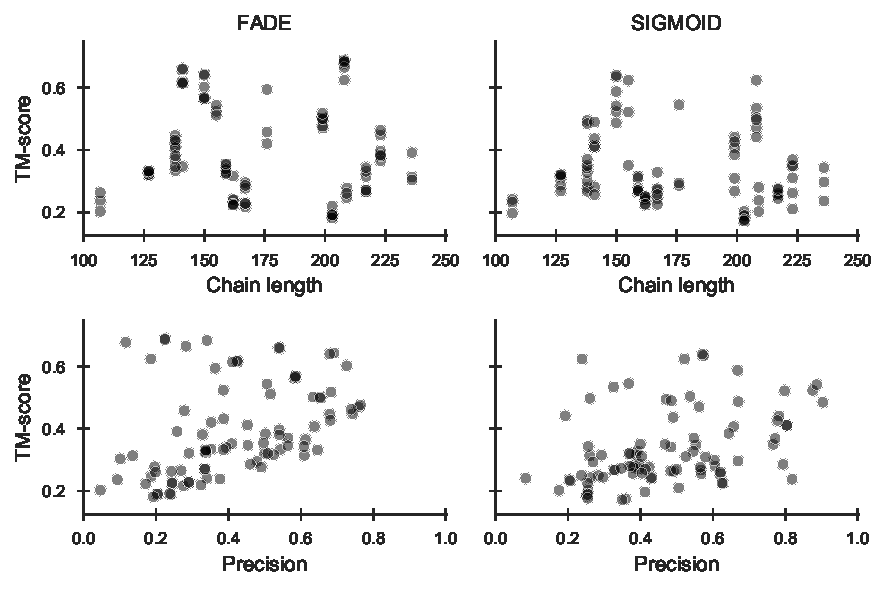
\includegraphics[width=\textwidth]{ample_predictors_tmsummary.pdf}
    \caption[Influence of target chain length and restraint precision on TM-score]{Effects of target chain length and restraint precision on the median TM-score for FADE and SIGMOID ROSETTA energy functions. Each scatter point represents a 1,000-decoy set.}
    \label{fig:ample_predictor_tmsummary}
\end{figure}

\subsection{Impact of metapredictors and energy functions on AMPLE}
The results obtained from the decoy quality comparison outlined in the previous section highlighted differences between the FADE and SIGMOID ROSETTA energy functions. This difference was more pronounced for some targets and did not generalise well in favour of one energy function. Thus, the next step in this study was to analyse the consequences  of these differences for unconventional \gls{mr} using the automated pipeline AMPLE.

Overall, the decoys restrained with GREMLIN distance restraints via the SIGMOID energy function throughout the \textit{ab initio} protein structure prediction process yielded six out of 18 possible structure solutions (\cref{fig:ample_predictor_ample}). This result was the highest of all trialled conditions and only resulted in one more structure solution compared to unrestrained ROSETTA decoys. All remaining conditions resulted in fewer structure solutions than those from ROSETTA decoys. Furthermore, the conditions METAPSICOV (FADE function), METAPSICOV BBCONTACTS (FADE function) and PCONSC2 BBCONTACTS (FADE function) yielded no more than half of the structure solutions achieved by GREMLIN (SIGMOID function). The remaining two conditions --- PCONSC2 (FADE function) and GREMLIN+BBCONTACTS (FADE function) --- resulted in four out of 18 structure solutions. The addition of BBCONTACTS did not improve decoy quality enough to increase the chances of structure solution success; however, the structure of the bovine peptide methionine sulfoxide reductase (\gls{pdb}: 1fvg) was only solved with the GREMLIN+BBCONTACTS (FADE function) decoys further supporting the small but important value of BBCONTACTS restraint addition to separately determined contact predictions.

\begin{figure}[H]
    \centering
    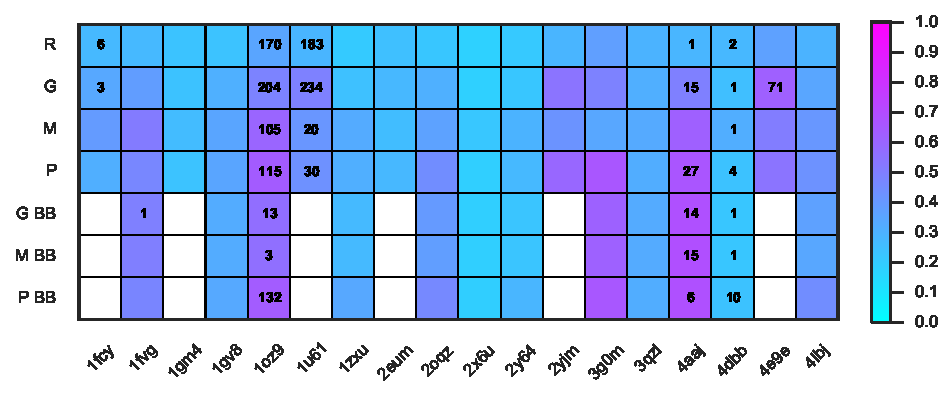
\includegraphics[width=\textwidth]{ample_predictors_ample.pdf}
    \caption[Structure solution count forom AMPLE-derived search models]{Structure solution count for AMPLE search models generated from decoys with varying contact prediction and ROSETTA energy function conditions: unrestrained ROSETTA (R); GREMLIN (G; SIGMOID function); METAPSICOV (M; FADE function); PCONSC2  (P; FADE function); GREMLIN+BBCONTACTS (G BB; FADE function); METAPSICOV+BBCONTACTS (M BB; FADE function); PCONSC2+BBCONTACTS (P BB; FADE function). The colour scale of each square indicates the median TM-score of all 1,000 starting decoys.}
    \label{fig:ample_predictor_ample}
\end{figure}

The number of structure solutions obtained from the decoy sets subjected to the AMPLE pipeline were somewhat surprising given that ROSETTA decoys resulted in the second-most structure solutions. These results suggested that AMPLE was unable to exploit the true value of more accurate decoy sets. This hypothesis was further supported when considering the decoy set quality and the number of structure solutions (\cref{fig:ample_predictor_ample}). For example, PCONSC2 (FADE function) decoys predicted for the hypothetical protein AQ\_1354 (\gls{pdb}: 1oz9) showed high accuracy, and thus would generally be considered highly desirable starting structures for the AMPLE protocol. Nevertheless, the AMPLE protocol was unable to exploit these decoys for successful \gls{mr} structure solution. Similarly, the high-accuracy contact-assisted decoys sets predicted for other targets, e.g. cysteine desulferation protein SufE (\gls{pdb}: 3g0m; median TM-score PCONSC2+BBCONTACTS (FADE function)=0.661) also failed to result in \gls{mr} solutions. In comparison, the median TM-scores for all successful ROSETTA decoy sets did not exceed 0.355 TM-score units, which suggested that the AMPLE routine may be optimised for less accurate ROSETTA decoys.

Naturally, one would expect the best decoys to result in the most accurate ensemble search models, which in turn yield the highest number of structure solutions per target. However, here we demonstrated that the most accurate decoys did not guarantee structure solution, and in contrast some poorly predicted decoy sets achieved structure solution. Thus, it was essential to investigate the stage in AMPLE's cluster-and-truncate approach at which the higher decoy quality resulted in less suitable ensemble search models for \gls{mr}.

\begin{figure}[H]
    \centering
    \begin{subfigure}[b]{0.49\textwidth}
        \centering
        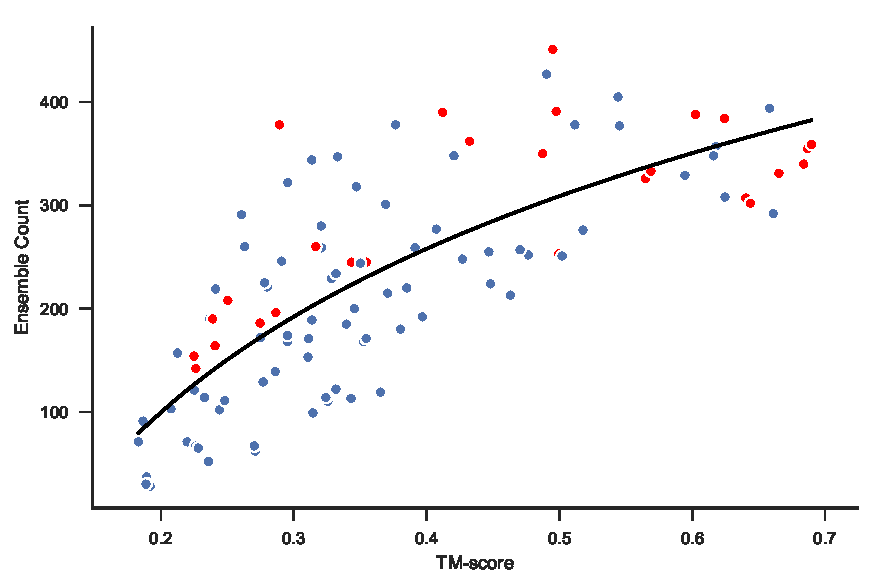
\includegraphics[width=\textwidth]{ample_predictors_ensdep.pdf}
        \caption{}
        \label{fig:ample_predictor_ensdep}
    \end{subfigure}
    %
    \begin{subfigure}[b]{0.49\textwidth}
        \centering
        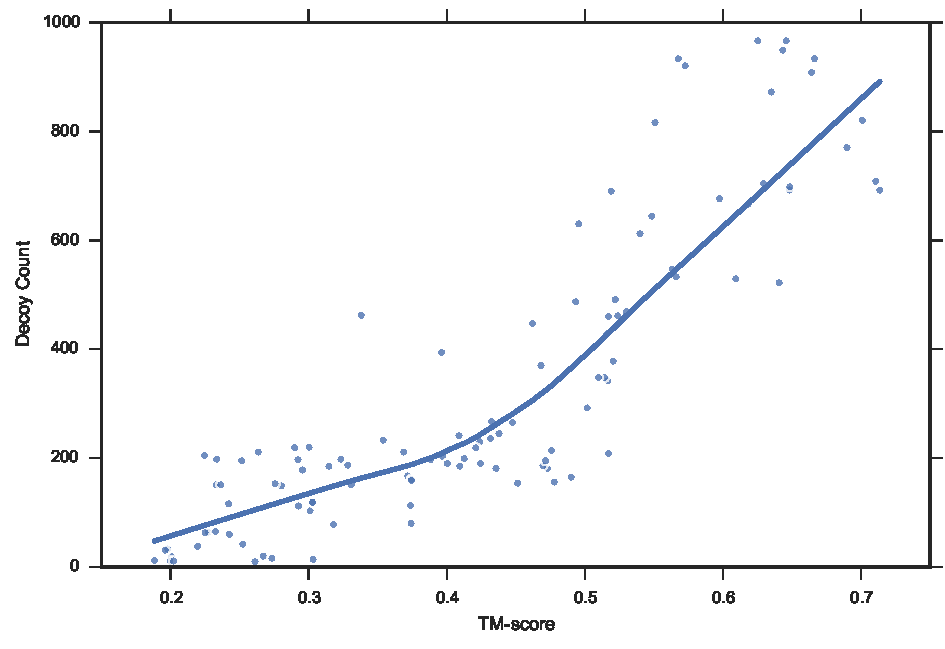
\includegraphics[width=\textwidth]{ample_predictors_clusizetm.pdf}
        \caption{}
        \label{fig:ample_predictor_clusizetm}
    \end{subfigure}

    \caption[Relationship between TM-score, AMPLE search model size and SPICKER cluster count]{(a) Comparison of median TM-score (per 1,000 decoys) against the resulting AMPLE ensemble search model count. The equation of the line of best fit is defined by $y=228.50*\ln\left(20.96*x\right)-227.95$. Red dots indicate successful ensemble sets. (b) Relationship between cluster median TM-score and the number of cluster decoys. Blue line represents line of best fit with equation $y=148.85*\exp\left(2.90*x\right)-225.76$.}
\end{figure}

The data generated as part of this study reveale a positive correlation ($\rho_{Spearman}=0.78$; $p<0.001$) between the decoy quality and the number of resulting AMPLE ensemble search models. In \cref{fig:ample_predictor_ensdep}, the plotted data alongside a line of best fit further illustrate that small differences in decoy quality in the lower TM-score regions increased the total number of generated ensemble search models dramatically. However, once the threshold of 0.5 TM-score units was surpassed the number of generated ensemble search models plateaued at around ~350-400 ensemble search models, approaching the maximum number of search models generatable by AMPLE. Furthermore, the data suggested that sets containing fewer than 100 ensemble search models did not lead to structure solution, although this result needed to be considered with care given the difficulty of predicting which search model will lead to structure solution.

\begin{figure}[H]
    \begin{subfigure}[b]{\textwidth}
        \centering
        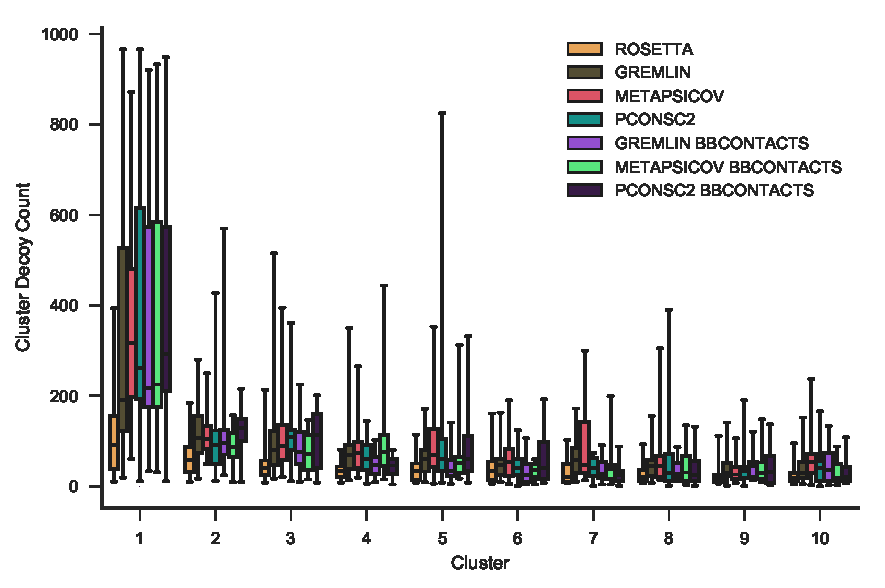
\includegraphics[width=0.9\textwidth]{ample_predictors_clusize.pdf}
        \caption{}
        \label{fig:ample_predictor_clusize}
    \end{subfigure}

    \begin{subfigure}[b]{\textwidth}
        \centering
        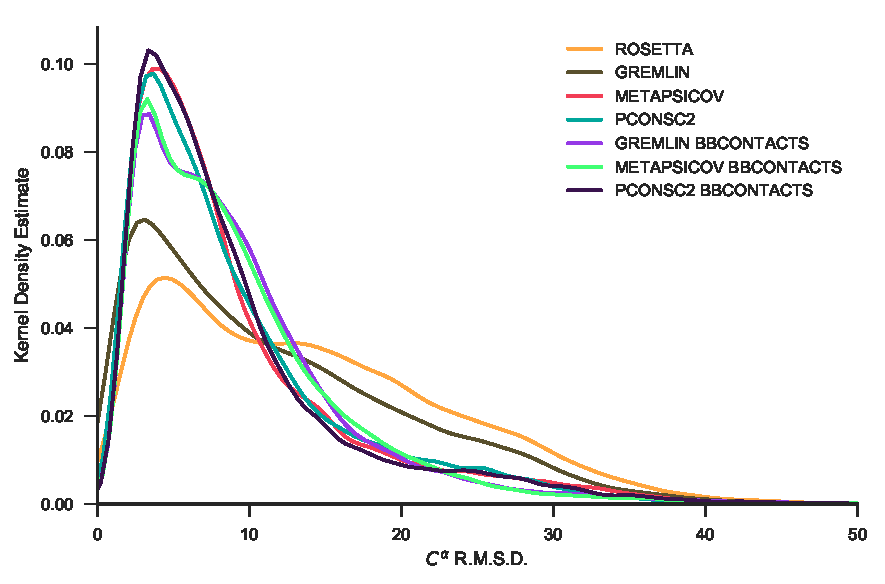
\includegraphics[width=0.9\textwidth]{ample_predictors_carmsd.pdf}
        \caption{}
        \label{fig:ample_predictor_carmsd}
    \end{subfigure}
    \caption[Effects of decoy sets on SPICKER clustering]{(a) SPICKER cluster sizes of each target grouped the restraint condition used during the structure prediction protocol. Whiskers span the range from the minimum to maximum counts. (b) \Gls{kde} of C\textalpha\ interatomic \gls{rmsd} for SPICKER clusters.}
\end{figure}

Besides looking at the relationship between entire decoy sets and the resulting structure solutions on a per-target or per-condition basis, it was important to also consider individual ensemble search models, their origins and their properties in relation to \gls{mr} metrics. Findings outlined in \cref{chap:proof_of_principle} highlighted the relationship between the number of decoys in the first cluster and its decoy quality (see \cref{chap:proof_of_principle}). Here, further support for these findings was given by means of the positive relationship between the median TM-scores and the corresponding size of the largest SPICKER cluster (\cref{fig:ample_predictor_clusizetm}). An analysis of the cluster sizes demonstrated the downstream benefits of increased decoy quality through contact restraints in the folding process (\cref{fig:ample_predictor_clusize}). The sizes of the first three clusters generated from most contact-restraint decoy sets greatly surpassed their equivalent cluster sizes for unrestrained ROSETTA decoys. Given that cluster sizes correlated with decoy quality, these results also supported the idea that the mean C\textalpha\ \gls{rmsd} --- as calculated by THESEUS for cluster truncation --- was directly related to better decoy quality via the larger number of decoys in each cluster (\cref{fig:ample_predictor_clurmsd}). The same mean C\textalpha\ \gls{rmsd} was also related to the number of ensemble search models generated after subclustering (\cref{fig:ample_predictor_rmsdsm}), which hinted towards a direct relationship between increased quality of 1,000 decoys per set and the total number of ensemble search models generated. Interestingly, GREMLIN decoys showed similar C\textalpha\ \gls{rmsd} per cluster compared to unrestrained ROSETTA decoys (\cref{fig:ample_predictor_carmsd}), unlike all other contact-restraint-guided structure predictions. However, it is worth noting that almost no distinction could be made amongst the remaining contact restraint treatments despite some differences in cluster size distributions exist (\cref{fig:ample_predictor_clusize}).

\begin{figure}[H]
    \centering
    \begin{subfigure}[b]{0.49\textwidth}
        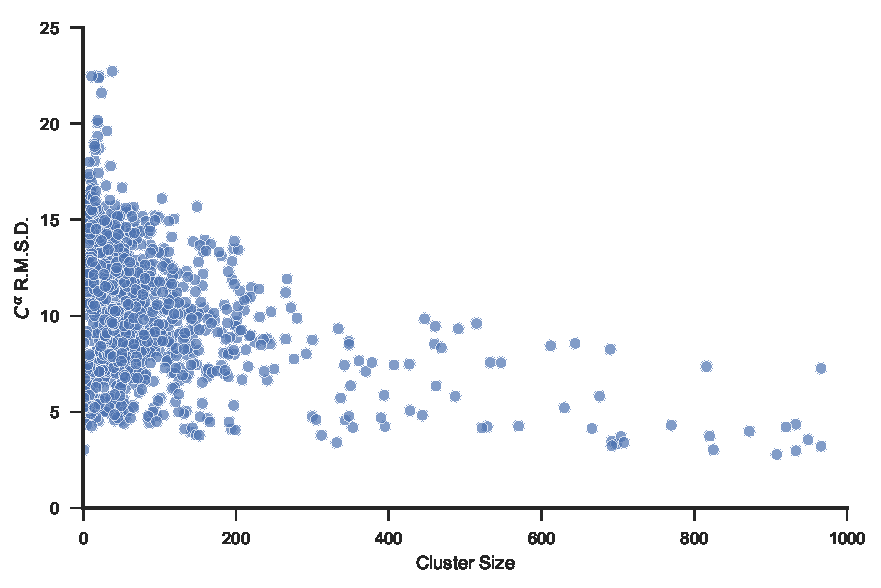
\includegraphics[width=\textwidth]{ample_predictors_clurmsd.pdf}
        \caption{}
        \label{fig:ample_predictor_clurmsd}
    \end{subfigure}
    % 
    \begin{subfigure}[b]{0.49\textwidth}
        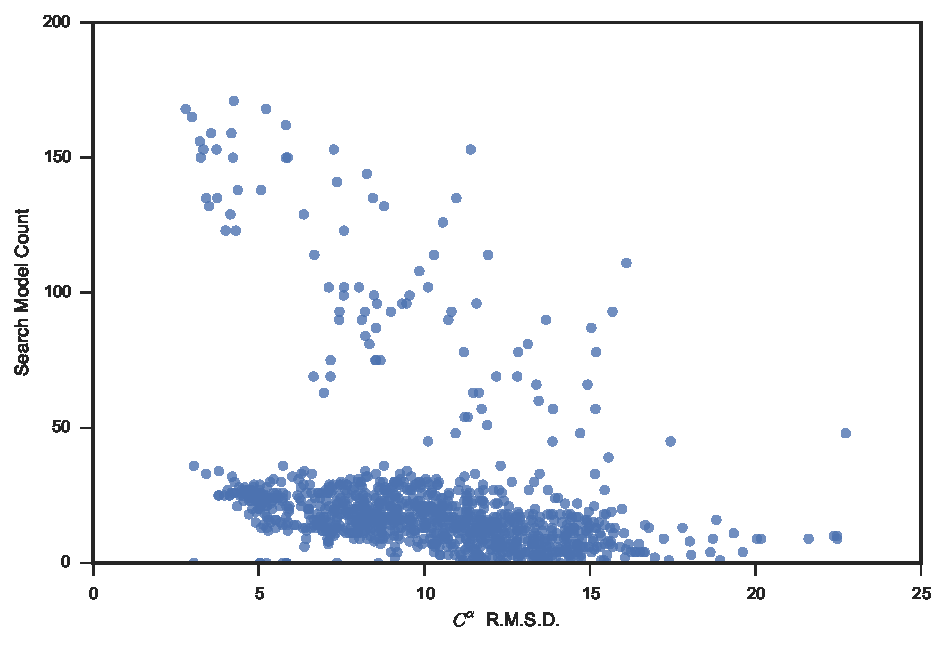
\includegraphics[width=\textwidth]{ample_predictors_rmsdsm.pdf}
        \caption{}
        \label{fig:ample_predictor_rmsdsm}
    \end{subfigure}

    \caption[SPICKER cluster properties]{(a) Number of decoys per SPICKER cluster plotted against the mean C\textalpha-atom \gls{rmsd} for all decoys in each cluster. (b) Mean C\textalpha-atom \gls{rmsd} for decoys per cluster plotted against the number of search models derived from the cluster.}
\end{figure}

The structure solution through pipelines like AMPLE and other unconventional \gls{mr} software \cite{Rodriguez2012-ad,Sammito2013-ug} can result from the placement of generated (ensemble) search models either in- or out-of-sequence register. The RIO metric \cite{Thomas2015-wu} can reliably assess the register placement, and thus was used to analyse the \gls{mr} placements of all search models of the seven targets with structure solutions from one or more decoy sets. The RIO scores for the hypothetical protein AQ\_1354 (\gls{pdb}: 1oz9) strongly supported the high quality decoys used as input across all seven contact conditions (\cref{fig:ample_predictor_riotar}). Most search models were placed in-register and hardly any search models with out-of-register RIO scores failed either. In contrast, the search models of N-(5’-phosphoribosyl)anthranilate isomerase (\gls{pdb}: 4aaj) --- derived from high quality decoys in most conditions --- showed a low percentage of AMPLE search models with RIO scores leading to structure solution (\cref{fig:ample_predictor_riotar}). Furthermore, the RIO scores normalized by the target chain length indicated that search models, independent of \gls{mr} structure solution, were relatively small only exceeding 20\% of the total target sequence in a few cases. 

\begin{figure}[H]
    \centering
    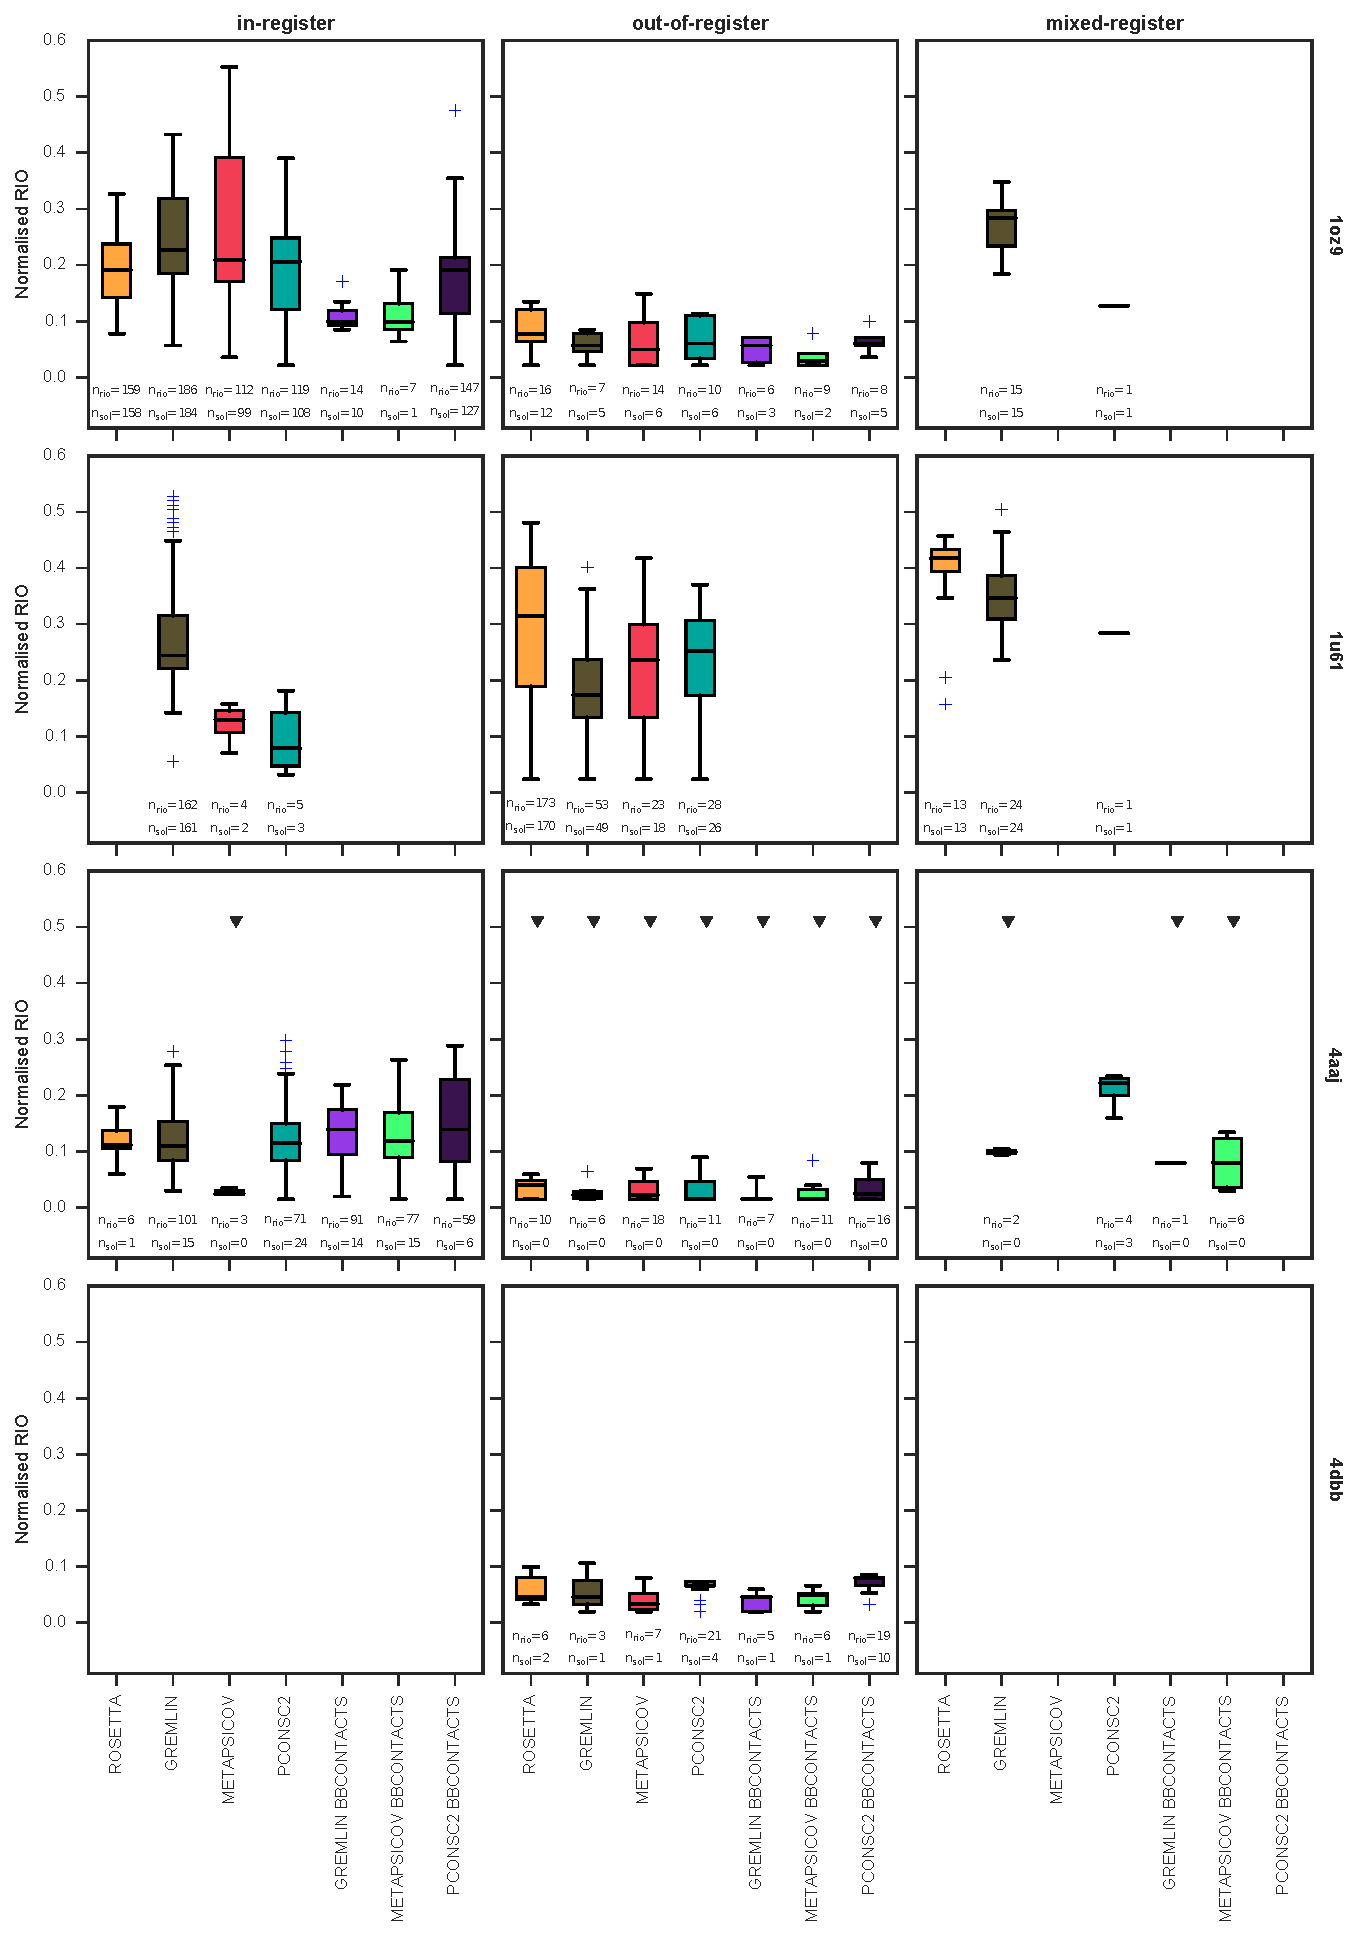
\includegraphics[width=0.95\textwidth]{ample_predictors_riotar.pdf}
    \caption[RIO score analysis of successful targets]{Normalised RIO score analysis of four successful targets in the \gls{mr} dataset. Black triangles indicate AMPLE search model sets without a structure solution.}
    \label{fig:ample_predictor_riotar}
\end{figure}

One interesting target in this set with respect to the sequence register of the AMPLE search models leading to structure solution was the putative ribonuclease III (\gls{pdb}: 1u61) domain. Although decoys from all contact conditions readily solved this target with at least 20 or more AMPLE search models, one important aspect arose from the RIO register analysis. Only GREMLIN decoys were primarily placed in-register (\cref{fig:ample_predictor_riotar}). AMPLE search models derived from the other three contact conditions, and in particular those from ROSETTA decoys, wereprimarily placed out-of-register with sequence coverage values of roughly 25\%. A close analysis of the diversity of AMPLE search models highlighted the accuracy of GREMLIN search models which represented a closely-matched substructure of the target protein (\cref{fig:ample_predictors_1u61_c2_t70_r1_reliable}).  

\begin{figure}[H]
    \begin{subfigure}[b]{0.49\textwidth}
        \centering
        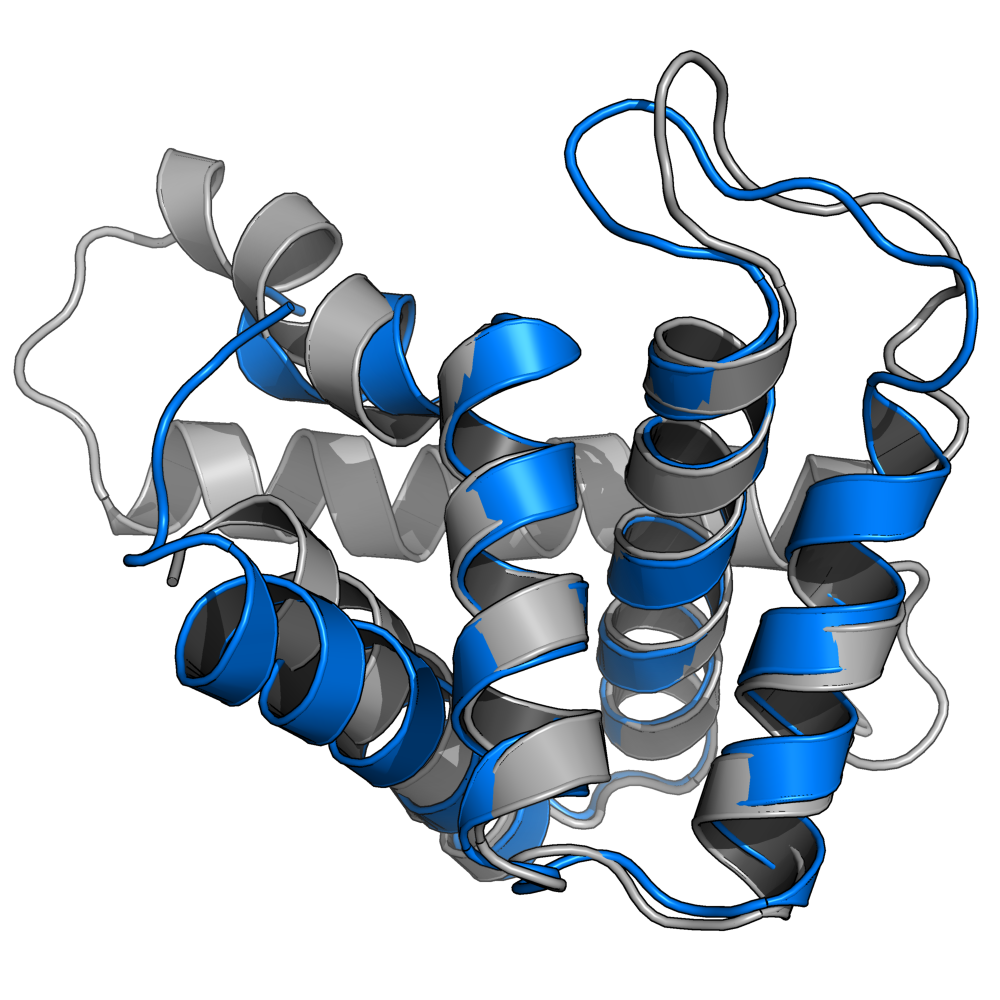
\includegraphics[width=0.8\textwidth]{ample_predictors_1u61_c2_t70_r1_reliable.png}
        \caption{}
        \label{fig:ample_predictors_1u61_c2_t70_r1_reliable}
    \end{subfigure}
    %
    \begin{subfigure}[b]{0.49\textwidth}
        \centering
        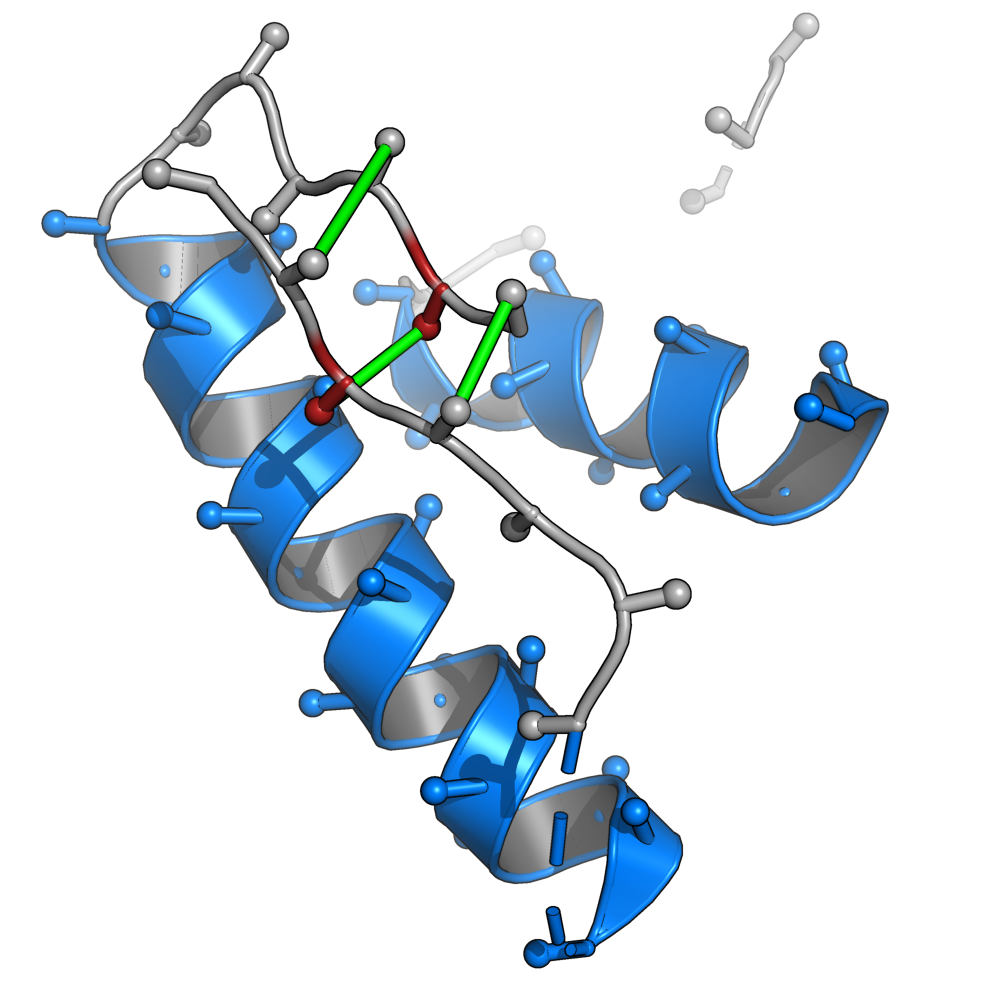
\includegraphics[width=0.8\textwidth]{ample_predictors_1fvg_gbb_phaser_c1_t25_r3_polyAla.png}
        \caption{}
        \label{fig:ample_predictors_1fvg_gbb_phaser_c1_t25_r3_polyAla}
    \end{subfigure}
    \caption[Examples of successfully placed AMPLE search models]{AMPLE ensemble search models post-PHASER placement for (a) putative ribonuclease III (\gls{pdb}: 1u61) and (b) peptide methionine sulfoxide reductase (\gls{pdb}: 1fvg). Search models (blue) are superposed to their native crystal structures (grey). BBCONTACTS distance restraints are represented as green lines. Secondary structure assignment calculated with STRIDE \cite{Frishman1995-si}. In (b), red residues indicate \textbeta-strand residues.}
\end{figure}

Compared to all other targets with structure solutions in at least one condition, the PTB domain of Mint1 (\gls{pdb}: 4dbb) produced similarly interesting yet somewhat surprising results. None of the search models, independent of their decoy source, had any residues placed in-register. All structure solutions were obtained from out-of-register search model placements (\cref{fig:ample_predictor_riotar}). A visual inspection of all successful search models revealed that structure solutions were exclusively obtained with idealised fragments. ROSETTA, GREMLIN and METAPSICOV decoys resulted in one or more single-helix ensemble search models that led to structure solution (\cref{fig:ample_predictors_4dbb_esm_egs}). More interestingly though, PCONSC2, GREMLIN+BBCONTACTS, METAPSICOV+BBCONTACTS and PCONSC2+BBCONTACTS decoys yielded one or more two-strand \textbeta-sheets which, after successful \gls{mr}, yielded fully built structures (\cref{fig:ample_predictors_4dbb_esm_egs}).

\begin{figure}[H]
    \centering
    \includegraphics[width=\textwidth]{ample_predictors_4dbb_esm_egs.png}
    \caption[Example of successfully placed AMPLE search model]{Successful search models post-PHASER placement (blue) superposed to the reference crystal structure (grey) for PTB domain of Mint1 (\gls{pdb}: 4dbb).}
    \label{fig:ample_predictors_4dbb_esm_egs}
\end{figure}

Lastly, three targets were solved with one or two decoy sets alone. The structures of the retinoic acid nuclear receptor HRAR (\gls{pdb}: 1fcy) and the peptide methionine sulfoxide reductase (\gls{pdb}: 1fvg) were only solved with a handful of AMPLE search models. Often singleton solutions like these are achieved through AMPLE's cluster-and-truncate procedure producing a single, idealised helix as search model. Here, the data confirmed this for target 1fcy, whereby single out-of-register helices derived from ROSETTA and GREMLIN decoys achieved structure solutions. However, the singleton search model derived from the GREMLIN+BBCONTACTS decoys for the peptide methionine sulfoxide reductase (\gls{pdb}: 1fvg) was placed in-register. A closer inspection of this AMPLE ensemble search model highlighted a great success of the approach of adding BBCONTACTS distance restraints to separately predicted base contact maps. In this instance, the successful AMPLE ensemble search model had 77\% of its 49 residues placed in-register. More importantly, the search model was made up of two \textbeta-strands packing against each other, which was supported by BBCONTACTS predictions (\cref{fig:ample_predictors_1fvg_gbb_phaser_c1_t25_r3_polyAla}). The last case, glycosylase domain of MBD4 (\gls{pdb}: 4e9e), solved solely with GREMLIN decoys yielding 71 structure solutions. All successful AMPLE search models derived from the GREMLIN decoys were placed in-register.

\section{Discussion}
This study was designed to explore the state-of-the-art metapredictor pipelines for residue-residue contact prediction. The main focus of this work was to distinguish differences in three key parts: raw contact predictions, their use in  \textit{ab initio} structure prediction and finally the effects on unconventional \gls{mr} using AMPLE.

Key findings in this study revealed METAPSICOV and PCONSC2 metapredictors to yield the most precise contact predictions regardless of target fold or size. These results are in line with previous findings, which independently confirmed METAPSICOV contact predictions to yield the highest precision across numerous prediction algorithms \cite{Wuyun2016-hh, De_Oliveira2017-gj}. However, work in this study cannot confirm their findings, which demonstrated more precise contact predictions for all-\textbeta\ and mixed \textalpha-\textbeta\ protein targets compared to all-\textalpha\ ones. Several reasons might give insights into this discrepancy: (1) a much smaller sample size was trialled in this study (\textcite{Wuyun2016-hh}: 680; \textcite{De_Oliveira2017-gj}: ~3500); (2) the targets were chosen to deliberately sample various alignment depths including relatively low alignment depth ($<200$) values; (3) only final contact predictions were analysed, thus benefiting from post-prediction consensus finding and contact map processing through unsupervised machine-learning algorithms.

Furthermore, the results obtained in this study demonstrated that two similar ROSETTA energy functions yield different structure prediction results. The FADE function on average achieves more accurate structure predictions compared to the SIGMOID one. This result seems striking at first; however, a closer inspection of each of the energy function parameters gives possible insights into the reasons for the different outcomes. The FADE energy function defines both a maximum and minimum distance. The FADE energy function also does not consider amino acid-specific distances while the SIGMOID function does \cite{Kamisetty2013-le}. Furthermore, a custom weight factor is added for SIGMOID restraints to balance the restraint term in the overall energy term of each decoy (Sergey Ovchinnikov, personal communication). Thus, small changes in each of those definitions could have significant effects on the final structure prediction. Unfortunately, it is out of the scope of this study to explore all variations, and thus results aid primarily as guide for future work and AMPLE users. This study highlighted again the benefits of adding BBCONTACTS predictions to existing contact maps to further restrain \textbeta-rich regions during \textit{ab initio} protein structure prediction. 

Lastly, part of the comparison carried out in this study was aimed specifically at \gls{mx} experimentalists and, in particular, AMPLE users. Beyond the proof-of-principle study described in \cref{chap:proof_of_principle}, this work further illustrated how important additional restraint information is to increase the chances of unconventional \gls{mr} success. However, this work also highlighted limitations in the AMPLE routine whereby decoys that were restrained by predicted residue-residue contacts achieved much higher decoy quality compared to unrestrained ROSETTA decoys, yet solved fewer targets. The idea that restrained decoys might benefit from a different kind of processing was further supported by the most successful decoy sets, which were obtained with GREMLIN contact predictions. Given that GREMLIN and ROSETTA decoys achieved similar decoy qualities across multiple targets, their structure solutions were identical for all of ROSETTA's successful solutions. GREMLIN decoys outperformed ROSETTA decoys solely on the basis that it acquired highly accurate decoys for one further target, and thus achieved the most structure solutions in this study. 

Therefore, further work was required to identify the optimal strategy for decoy sets with high structural similarities to the native fold. Such work could focus on the recent idea of selecting decoys based on their long-range contact precision \cite{De_Oliveira2017-gj, Ovchinnikov2017-nd} to specifically eliminate the worst decoys, and thus enhance a more fine-grained clustering approach in SPICKER (\cref{chap:ample_decoys}). Alternatively, truncation could be guided by alternative means, such as the importance of each residue in the predicted contact map. Ultimately, it is key to improve the AMPLE protocol to exploit the much higher decoy quality to enhance the user’s chance of success.
